\documentclass{article}

\usepackage{graphicx}
\usepackage{tikz}
\usepackage{tikzsymbols}
\usetikzlibrary{calc,patterns,shapes.geometric}
\pagestyle{empty}
\usepackage[margin=0pt]{geometry}
\geometry{papersize={14in,12in}}

\def\centerarc[#1](#2)(#3:#4:#5){\draw[#1] ($(#2)+({#5*cos(#3)},{#5*sin(#3)})$) arc (#3:#4:#5);}

\begin{document}
	\begin{figure}
		\centering
		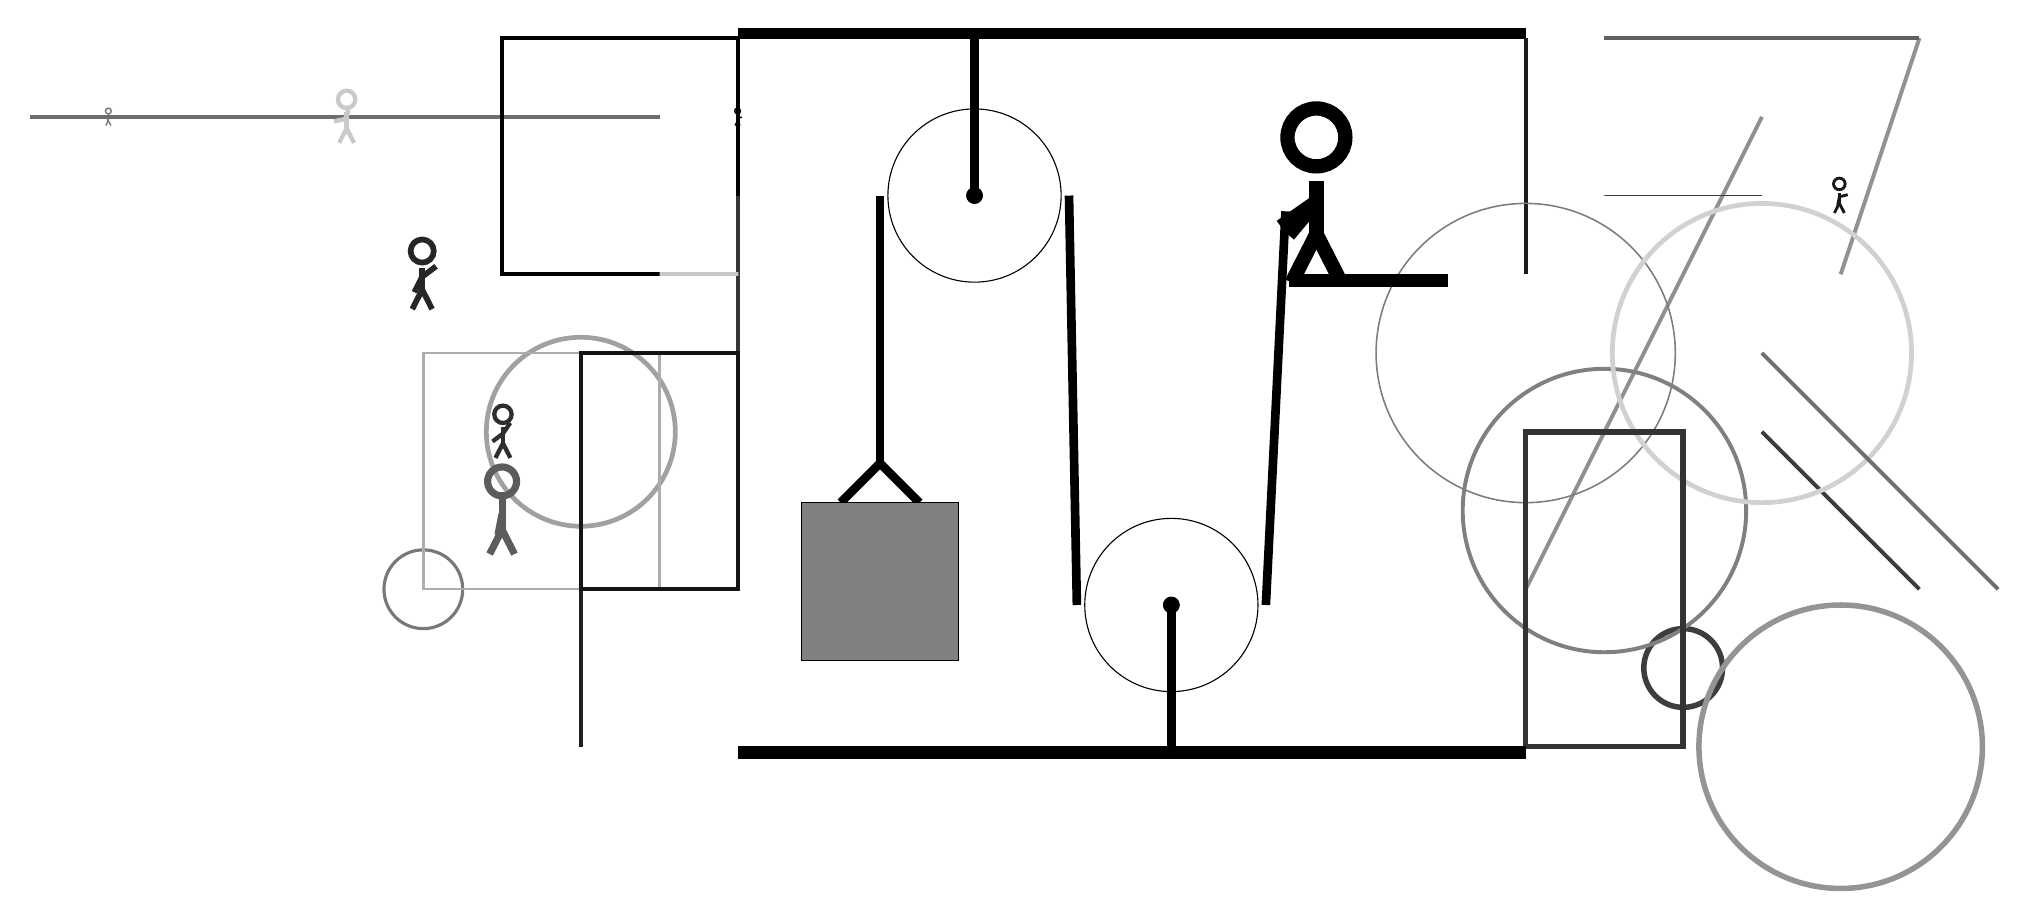
\begin{tikzpicture}
			%%%%% START %%%%%
			
			\draw[fill=black] (-2, 9) rectangle (8, 9.125);
			
			\draw (3.5, 1.8) circle (1.1);
			\draw[fill=black] (3.5, 1.8) circle (0.1);
			\draw[line width=1.1mm] (3.5, 1.8) -- (3.5, 0);
			
			\draw (1, 7) circle (1.1);
			\draw[fill=black] (1, 7) circle (0.1);
			\draw[line width=1.1mm] (1, 9) -- (1, 7);
			
			\draw [line width=0.4mm, color=black!53](-6, 2) circle (0.5);
			
			\draw[line width=0.5mm, color=black!43](8, 2) -- (11, 8);
			\draw[line width=0.2mm, color=black!76] (9, 7) rectangle (11, 7);
			\draw [line width=0.6mm, color=black!37](-4, 4) circle (1.2);
			\node[line width=0.3mm, color=black!85] at (-6, 6) {\Strichmaxerl[4][63][37]};
			\node[line width=0.5mm, color=black!53] at (-10, 8) {\Strichmaxerl[1][78][86]};
			
			\draw [line width=0.7mm, color=black!76](10, 1) circle (0.5);
			\draw[line width=0.5mm, color=black!89](8, 6) -- (8, 9);
			\draw[line width=0.5mm, color=black!57](-3, 8) -- (-11, 8);
			\draw[line width=0.5mm, color=black!43](13, 9) -- (12, 6);
			\draw[line width=0.5mm, color=black!77](11, 4) -- (13, 2);
			
			\draw [line width=0.2mm, color=black!51](8, 5) circle (1.9);
			\draw [line width=0.5mm, color=black!50](9, 3) circle (1.8);
			
			\draw[line width=0.5mm, color=black!100] (-2, 9) rectangle (-5, 6);
			\node[line width=0.6mm, color=black!100] at (-2, 8) {\Strichmaxerl[1][90][1]};
			\draw [line width=0.6mm, color=black!18](11, 5) circle (1.9);
			
			\node[line width=0.3mm, color=black!91] at (12, 7) {\Strichmaxerl[2][79][14]};
			
			\draw[line width=0.5mm, color=black!79](-2, 3) -- (-2, 7);
			\draw[line width=0.5mm, color=black!22] (-3, 6) rectangle (-2, 6);
			
			\draw[line width=0.5mm, color=black!88](-4, 5) -- (-4, 0);
			\draw[line width=0.7mm, color=black!80] (8, 4) rectangle (10, 0);
			
			\draw [line width=0.3mm, color=black!80](13, 3) circle (0.0);
			\draw[line width=0.3mm, color=black!32] (-3, 2) rectangle (-6, 5);
			\draw[line width=0.5mm, color=black!62](13, 9) -- (9, 9);
			\node[line width=0.5mm, color=black!21] at (-7, 8) {\Strichmaxerl[3][12][80]};
			
			\draw[line width=0.5mm, color=black!57](11, 5) -- (14, 2);
			\draw [line width=0.7mm, color=black!42](12, 0) circle (1.8);
			\node[line width=0.3mm, color=black!64] at (-5, 3) {\Strichmaxerl[5][79][90]};
			\draw[line width=0.5mm, color=black!92] (-4, 2) rectangle (-2, 5);
			\node[line width=0.5mm, color=black!82] at (-5, 4) {\Strichmaxerl[3][37][56]};
			
			\draw[line width=1.1mm](-0.7, 3.1) --  (-0.2, 3.6) -- (0.3, 3.1);
			\draw[fill=black!50] (-1.2, 3.1) rectangle (0.8, 1.1);
			
			\draw[line width=1.1mm](-0.2, 7) -- (-0.2, 3.6);
			\centerarc[line width=1.1mm](1, 7)(180:0:1.2000000000000002)
			\draw[line width=1.1mm](2.2, 7) -- (2.3, 1.8);
			\centerarc[line width=1.1mm](3.5, 1.8)(180:360:1.2000000000000002)
			\draw[line width=1.1mm](4.7, 1.8) -- (4.95, 6.8);
			
			\node at (5.3, 7) {\Strichmaxerl[10][35][-130]};
			\draw[fill=black] (5, 6) rectangle (7, 5.85);
			
			\draw[fill=black] (-2, 0) rectangle (8, -0.15);
			
			%%%%% END %%%%%
		\end{tikzpicture}
	\end{figure}	
\end{document}